\chapter{The Standard Model of Particle Physics}
\label{chap:theory}

%\chapterquote{}{}

\section{Introduction}

The standard model (SM) of particle physics is a quantum field theory
description of the fundamental particles of matter and their interactions. The
SM has been widely successful in its predictions, falling short in providing a
dark matter candidate, including the existence of neutrino oscillations and
incorporating gravitational interactions, among other possible discrepancies.
Nevertheless, it is the current best minimal description unifying the
electromagnetic, weak and strong forces. In the quantum field theory, the
equations of motion are determined from the Lagrangian through the principle
of least action. Gauge theories provide the mathematical basis to embed
physical symmetries within the model. 

The SM has had many distinguishing successes since its conception. One of
the most notable is the prediction of the Higgs boson
\cite{PhysRevLett.13.321,PhysRevLett.13.508,PhysRevLett.13.585} and its
subsequent discovery by the ATLAS \cite{Aad:2012tfa} and CMS
\cite{Chatrchyan:2012xdj} experiments. The Higgs field is crucial in providing
a mechanism for the apparent masses of the weak bosons, quarks and charged
leptons whilst maintaining a gauge invariant theory.

This chapter will include an overview of the properties of the SM with
particular detail on the quantum electrodynamic, quantum chromodynamic and
electroweak sectors, leading to a discussion of the spontaneous symmetry breaking in the SM, known as the Higgs mechanism. This is followed
by a discussion of the Monte Carlo techniques used to simulate the SM.


\section{Elementary particles}

The set of fundamental particles and interaction mediators within the SM is
shown in Fig.~\ref{fig:particle}. This includes the quarks --- fermion
constituents of protons and neutrons --- with three generations of up and
down-type quarks with a charge of $+2/3$ and $-1/3$ (in units of the
elementary charge). A quark also takes one of three colour states, the strong
force equivalent of the electric charge. Through these colour states the
quarks interact with the gluon colour octet via the strong interaction. In
addition, the lepton sector consists of charged fermions which, in addition to
the quarks, interact through the photon field leading to the electromagnetic
interaction. Furthermore, all fermions --- quarks, charged leptons and neutral
leptons (neutrinos) --- interact via the weak force, mediated by the \PW and
\PZ bosons. A set of antiparticles mirror all the fermions leading to 12
fermion fields and an equal number of anti-fermion fields, split into 6 quarks
and 6 leptons. 

\begin{figure}[htb]
    \centering
    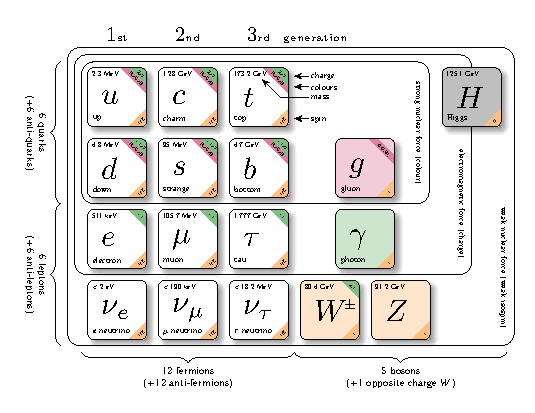
\includegraphics[width=0.8\textwidth]{diagrams/tikz/standard_model/standard_model.pdf}
    \caption[Summary of the standard model particles.]{
        Diagram of the particles within the SM including their quantum numbers such as charge, colour and spin, along with their measured masses. The left and right-handed chiral states are omitted and left for discussion in the main text.
    }
    \label{fig:particle}
\end{figure}


\section{Gauge theories}

In quantum field theory, the fundamental fields are unobservable. Instead,
properties deriving from these fields, such as the cross section or rate of an
interaction or decay, are measured. Many configurations of the underlying
fields can give identical observable quantities. The transformation between
these configurations is known as a gauge transformation and leaves the
physical observables unchanged, hence these transformations are known as gauge
invariant. Under Noether's theorem, a change in the field configuration which
leaves the action, and hence the Lagrangian density, invariant is associated
with conserved currents \cite{doi:10.1080/00411457108231446}. 

\subsection{Quantum Electrodynamics}

Quantum electrondynamics (QED) is a gauge theory that sets out to describe the
electron and the photon along with their interactions. The QED Lagrangian
density consists of a Dirac field, the electron; a vector field, the photon,
derived from Maxwell's equations; and an interaction term between the electron
and photon fields:
%
\begin{equation}
    \mathcal{L}_{\mathrm{QED}} = \mathcal{L}_{\mathrm{Dirac}} + \mathcal{L}_{\mathrm{Maxwell}}\ + \mathcal{L}_{\mathrm{int}}\ .
\end{equation}

Maxwell's equations of electromagnetism are obtained from the Euler-Lagrange
equations applied to the Lagrangian
%
\begin{equation}
    \mathcal{L}_{\mathrm{Maxwell}} = -\frac{1}{4}F^{\mu\nu}F_{\mu\nu}\ ,
\end{equation}
%
where $F^{\mu\nu}=\partial^{\mu}A^{\nu}-\partial^{\nu}A^{\mu}$
\cite{Peskin:1995ev} for the 4-potential $A^{\mu}$ with an electric scalar
potential time-like and magnetic vector potential space-like components.

The Dirac Lagrangian describes the equations of motion, through application of
the Euler-Lagrange equations \cite{Troutman1983}, of a spin-half fermion field
$\psi$. This field is represented as a four-component spinor which may be
interpreted as the spin-up and down of the left and right-handed helicity
states \cite{Peskin:1995ev}. To form Lorentz invariant quantities, required in
the Lagrangian, the adjoint field is defined as
$\bar{\psi}=\psi^{\dagger}\gamma^0$ where $\psi^{\dagger}$ is the Hermitian
conjugate of $\psi$ and $\gamma^0$ is the time-like component of the Dirac
gamma matrices. These matrices obey the anticommutation relation
$\{\gamma^{\mu},\gamma^{\nu}\} = 2g^{\mu\nu}$, where $g^{\mu\nu}$ is the
Minkowski space metric, leading to the Lorentz invariant quantities such as
$\bar{\psi}\psi$ and $\bar{\psi}\gamma^{\mu}\psi$ \cite{Peskin:1995ev}. These
quantities form the basis of the Dirac Lagrangian of a free spin-half fermion:
%
\begin{equation}
    \mathcal{L}_{\mathrm{Dirac}} = i\bar{\psi}\gamma^{\mu}\partial_{\mu}\psi - m\bar{\psi}\psi\ ,
\end{equation}
%
where $i\partial_{\mu}$ is the position-space representation of the 4-momentum
$p_\mu$, and $m$ is the mass of the particle \cite{1928RSPSA.117..610D}.
$U(1)$ group transformations of the field
%
\begin{equation}
    \psi \mapsto e^{i\alpha}\psi
\end{equation}
%
are not physical observables since they cancel in the magnitude of the matrix
element used to determine the rate or cross section of a process. The
Lagrangian is already invariant to such global transformations. However, local
transformations where $\alpha\mapsto\alpha(x)$ introduces a term to the Dirac Lagrangian given by
%
\begin{equation}
    \mathcal{L}_{\mathrm{Dirac}} \mapsto \mathcal{L}_{\mathrm{Dirac}}  - \bar{\psi}\gamma^{\mu}(\partial_\mu\alpha(x))\psi\ ,
\end{equation}
%
To enforce gauge invariance, this additional term must be removed by
introducing an additional field to the Dirac Lagrangian with a $U(1)$
transformation which opposes the additional term. Therefore, a $U(1)$ gauge
invariant electron field must include an interaction with this new field,
which is the photon field. This interaction term is
realised through gauge invariance as
%
\begin{equation}
    \mathcal{L}_{\mathrm{int}} = -g\bar{\psi}\gamma^{\mu}\psi A_{\mu}\ ,
\end{equation}
%
where $A_\mu$ transforms into $A_\mu - (\partial_\mu\alpha(x))/g$ under a
local phase transformation with a coupling constant $g$ between the
electron and photon interaction. The interaction term is absorbed into the
definition of a gauge covariant derivative $D_{\mu} \equiv \partial_\mu
+igA_\mu$ to give the full QED Lagrangian as
%
\begin{equation}
    \mathcal{L}_{\mathrm{QED}} = i\bar{\psi}\gamma^{\mu}D_{\mu}\psi - m \bar{\psi}\psi - \frac{1}{4}F^{\mu\nu}F_{\mu\nu}\ .
\end{equation}
%
Additional Dirac terms, with associated photon interactions, are included for
all spin-half charged fermions of the \SM.


\subsection{Quantum Chromodynamics}

The QED Lagrangian does not include self interaction terms with the photon
field $A_\mu$. The extension to include interactions of the form
$A^{\mu}A^\nu\partial_\mu A_\nu$ and $A^4$ introduces us to the theory of the
strong force --- quantum chromodynamics (QCD). QCD sets out to explain the
quarks, gluons and their interactions. The quark model explains the plethora
of mesons and baryons as bound states of two and three quarks, respectively.
These quarks have fractional electric charges of $+2/3$ and $-1/3$ with six
flavours. Furthermore, to explain the baryon spectrum with the Fermi exclusion
principle, one of three colour states is assigned to quarks with equivalent
anti-quark colour states \cite{Peskin:1995ev}. The minimal symmetry of which
the quark colour states may be invariant to belongs to the $SU(3)$ group.
Including the Dirac Lagrangian for the quark states and enforcing gauge
invariance requires countering field interaction terms, similar to the interaction between the electron and photon. An $SU(3)$
rotation is represented by eight $3\times 3$ matrices, hence eight counter
terms with an independent field are required. These represent the eight gluon
states $A_{\mu,a}$ with $a\in\{1,2,\ldots,8\}$. Therefore, the QCD Lagrangian
is given by
%
\begin{equation}
    \mathcal{L}_{\mathrm{QCD}} = i\bar{\psi}_f\gamma^{\mu}D_\mu\psi_f - m_f\bar{\psi}_f\psi_f - \frac{1}{4}F^{\mu\nu}_a F_{\mu\nu,a}\ ,
\end{equation}
%
where $\psi_f$ is the quark spinor state with flavour $f$. The covariant
derivative and field strength tensor are extended to gluon equivalents as
%
\begin{equation}
    D^{\mu} = \partial^\mu - i g_{s}A^\mu_a t_a
\end{equation}
%
and
%
\begin{equation}
    F^{\mu\nu}_a = \partial^\mu A^\nu_a - \partial^\nu A^\mu_a + g_{s} f_{abc}A^\mu_b A^\nu_c\ ,
\end{equation}
%
where $g_{s}$ is the quark-gluon coupling strength, $t_a$ are the generators
of the $SU(3)$ group and $f_{abc}$ appears from the non-commutative property
of the generators: $[t_a,t_b]=if_{abc}t_c$, leading to gluon self-interaction
vertices \cite{Peskin:1995ev}.

As a result of the QCD interactions the strong coupling constant $g_s$
decreases with the energy scale leading to two notable effects. The first is
weak strength of the strong force at high energies, allowing perturbative
calculations. Whereas at low energies the increasing strength leads to the
confinement of quarks and gluons, preventing the existence of isolated color
charged particles in normal conditions. This property is important in high
energy particle collisions where outgoing quarks and gluons form into showers
of hadrons, detected as a cone of hadronic activity \cite{Peskin:1995ev}.


\subsection{Electroweak physics}\label{sec:ew-theory}

Another realised symmetry is the invariance between up and down-type quarks.
However, this symmetry is broken by the weak force where left and right-handed
fermions are treated differently. Instead the left-handed up and down-type
quarks are symmetric under the weak interaction, grouped into doublets with an
$SU(2)$ symmetry, and similarly for right-handed antiparticles. However,
right-handed fermions and left-handed antifermions do not interact with the
weak force, and hence form a singlet with a $U(1)$ symmetry. Therefore, the
electroweak interaction is symmetric under $SU(2)\times U(1)$ transformations.
The modified covariant derivative requires three generators of the $SU(2)$
group and a single generator of the $U(1)$ group:
%
\begin{equation}
    D_\mu = \partial_\mu + i\frac{g}{2}W_\mu^i\sigma^i + g' Y_W B_\mu\ ,
\end{equation}
%
where $i$ labels the generators of the $SU(2)$ group, $2\times 2$ Pauli
matrices $\sigma^i$, with associated field $W_\mu^i$ and coupling $g$; and
$Y_W$ is the generator of the $U(1)$ group with the field $B_\mu$ and coupling
$g'$. The $W_\mu^i$ and $B_\mu$ fields represent the
physical photon, $W^{\pm}$, $Z^{0}$ bosons through the combinations \cite{Peskin:1995ev}
%
\begin{align}
    W_\mu^\pm & = \frac{1}{\sqrt{2}}\left(W_\mu^1 \mp i W_\mu^2\right)\ ,\\\nonumber
    Z^0_\mu & = \frac{1}{\sqrt{g^2+g'^2}}\left(g'W_\mu^3 + gB_\mu\right)\quad\mathrm{and}\\\nonumber
    A_\mu & = \frac{1}{\sqrt{g^2+g'^2}}\left(g'W_\mu^3 - gB_\mu\right)\ .
\end{align}
%
However, introducing mass terms for the \PW and \PZ bosons breaks the gauge
invariance of the Lagrangian. Similarly, the broken symmetry between left and
right-handed particles leads to gauge invariance breaking terms: $\hat{\psi}_L\psi_R$ and $\hat{\psi}_R\psi_L$, preventing quark mass terms. Instead, a process known as spontaneous
symmetry breaking gives rise to these mass terms whilst remaining as a gauge invariant theory.


\subsection{Spontaneous symmetry breaking}

The spontaneous symmetry breaking in the electroweak sector provides mass
terms for the \PW and \PZ bosons through the Higgs mechanism
\cite{PhysRevLett.13.321,PhysRevLett.13.508,PhysRevLett.13.585}. A Lorentz
scalar, isospin-doublet field $\phi$ obeying the $U(1)$ gauge symmetry is
introduced with a quartic potential
%
\begin{equation}
    \mathcal{L}_{\mathrm{Higgs}} = (D_\mu\phi)^*(D^\mu\phi) +\mu^2|\phi|^2 - \lambda|\phi|^4\ .
\end{equation}
%
The covariant derivate includes the weak fields for a gauge invariant Lagrangian. However, the vacuum expectation value of the field $\phi$ is non-zero and given by
%
\begin{equation}
    \langle \phi \rangle = \frac{1}{\sqrt{2}}
    \begin{pmatrix}
        0 \\ v
    \end{pmatrix}
\end{equation}
%
with $v^2=\mu^2/2\lambda$. The $\phi$ field can be rewritten in terms of two fields, $h$ and $\chi$, with no vacuum expectation values:
%
\begin{equation}\label{eq:phi}
    \phi = \frac{1}{\sqrt{2}}(v + h)e^{i\chi/v}\ .
\end{equation}
%
The vacuum state is symmetric in a $U(1)$ transformation, allowing for any
$\chi$ terms to be absorbed by a redefinition of the $U(1)$ gauge
transformation. Expanding out the Lagrangian with this redefinition introduces
$h$ as a real scalar field with mass terms for the $h$, \PW and \PZ bosons of
$\sqrt{2}\mu$, $gv/2$, and $(v/2)\sqrt{g^2+g'^2}$ respectively. The photon
does not acquire a mass term, as required for the SM.

Since the $\phi$ field is an $SU(2)$ doublet a gauge invariant coupling with
the left-handed lepton doublet $E_L$ and the right-handed singlet $e_R$ is
included in the Lagrangian as
%
\begin{equation}
    -\lambda_e (\bar{E}_L \phi) e_R + \mathrm{h.c.}\ ,
\end{equation}
%
where h.c. represents the Hermitian conjugate of the terms already present and
$\lambda_e$ is a new dimensionless coupling constant \cite{Peskin:1995ev}.
Again, expanding out the Lagrangian with Eq.~\ref{eq:phi} leads to lepton mass
terms with $m_e = \lambda_e v/\sqrt{2}$. Similarly, the equivalent $SU(2)$
invariant coupling for the left-handed quark doublet $Q_L$ and right-handed
singlets $d_R$ and $u_R$ is included in the Lagrangian as
%
\begin{equation}
    -\lambda_d (\bar{Q}_L\phi) d_R - \lambda_u \epsilon^{ab}(\bar{Q}_L\phi_b^{\dagger})u_R + \mathrm{h.c.}\ ,
\end{equation}
%
where $\epsilon^{ab}$ is a two-dimensional Levi-Civita tensor \cite{Peskin:1995ev}.
In a similar manner to the lepton fields, the quark fields acquire mass terms
with $m_d = \lambda_d v/\sqrt{2}$ and $m_u = \lambda_u v/\sqrt{2}$. Additional
generations of quarks introduce mixing terms between the various generations
of up and down-type quarks through \PW boson interactions with couplings
determined by the $3\times 3$ unitary Cabibbo-Kobayashi-Maskawa (CKM) mixing
matrix \cite{PhysRevLett.10.531,Kobayashi:1973fv}.

Neutrinos do not have a right-handed chiral state and hence no couplings to
the $\phi$ field can be included without breaking a gauge symmetry. Therefore,
the neutrinos are massless in the SM. However, the neutrino flavours mixing
has been measured experimentally and included ad hoc into the SM through the
Pontcorvo-Maki-Nakagawa-Sakata matrix\cite{Pontecorvo:1957qd,Maki:1962mu},
analogous to the CKM matrix.

In addition to the mass terms introduced through spontaneous symmetry breaking, the $h$ field couples to the \PW and \PZ with a coupling proportional to the fourth-power of their mass, to fermions to the square of their mass, along with a trilinear and quartic self coupling.


\section{Event simulation and generation}
% https://arxiv.org/pdf/1101.2599.pdf

The complexity involved with modern particle accelerators, colliders and detectors require the use of simulated events to interpret the results and validate our understanding of the SM and beyond. To avoid needlessly generating all possible events from a collision, only the processes of interest are simulated through Monte Carlo integration of multidimensional integrals to determine differential cross sections, and hence the scattering probabilities. Additional Monte Carlo techniques allow the sampling of these distributions to generate events.

Event simulation is based on perturbation theory where higher order diagrams are neglected in calculations to avoid expensive computations. However, ignoring the entire perturbation series leads to infrared and ultraviolet divergences \cite{Ellis:1991qj}. These are avoided through renormalisation techniques and introducing the factorisation $\mu_F$ and renormalisation $\mu_R$ scales. Physical observables should not depend on these quantities, however, limitations in the calculations lead to some dependence.


\subsection{Hadron collider physics}\label{sec:hadron-collider-physics}

In a proton-proton collider, the hard interaction cross section between parton
$a$ and parton $b$ in each proton is factorised into \cite{Ellis:1991qj}
%
\begin{equation}
    \sigma = \sum_{a,b} \int_0^1 dx_a dx_b \int f_a(x_a,\mu_F)f_b(x_b,\mu_F) d\hat{\sigma}_{ab\rightarrow n}(\mu_F,\mu_R)\ ,
\end{equation}
%
where $x_a$ is the proton momentum fraction associated to parton $a$ and $x_b$ for parton $b$ in the other proton. The $f(x,\mu)$ are the parton distribution function which describe the momentum fraction for a particular parton within a proton. The parton cross section $\hat{\sigma}_{ab\rightarrow n}$ denotes the interaction of partons $a$ and $b$ to form a specific $n$-particle final state. This is determined from a matrix element calculation integrated over the available phase space for the outgoing particles, averaged over initial spin and colour states and scaled by the parton flux. The number of Feynman diagrams used in the matrix element calculation is determined from the accuracy required. Leading order (LO) refers to the lowest power in the strong and electroweak coupling constants, which often refers to tree-level diagrams. Next-to-leading order (NLO) generators include the next lowest power, with the inclusion of higher-order virtual and real-emission corrections. Although the electroweak coupling constant is relatively small, virtual gauge boson loops result in logarithms \cite{Sudakov:1954sw} that scale with the ratio of the centre of mass energy to the weak scale ($\SI{100}{GeV}$), and hence become large corrections at a TeV colliders and beyond. The order to which these logarithms are calculated in the perturbation series proceeds from the leading logarithm (LL) to the next-to-leading logarithm (NLL), and so on.

The choice of $\mu_F$ and $\mu_R$ are typically set by the scale of the interaction, such as the mass of an s-channel resonance, or transverse momentum of the primary outgoing particle. The scale of the interaction may also have further meaning on the initial and final-state parton showers, where care is taken to avoid double-counting particles between the matrix element calculation and parton showering. The impact of the choice of scale is determined by varying both $\mu_F$ and $\mu_R$ up and down by a factor, both uncorrelated and fully correlated. This rescaling is provided as an alternative event weight to propagate as a systematic uncertainty.

The parton distribution functions are typically determined from a fit between data and theory predictions. The evolution of these functions from low momentum scale measurements to energy frontiers is given by the DGLAP equations \cite{Altarelli:1977zs,Dokshitzer:1977sg,Gribov:1972ri}. The uncertainties associated with these measurements are propagated through to the generated events.

The fixed order calculations discussed are not sufficient at encapsulating the full picture of the scattering process. Higher order effects are included through parton showering where the fragmentation of partons is simulated, down to the hadronization at $\SI{1}{GeV}$ scales. This hadronization process confines coloured particles into bound neutral final states, typically resulting in a shower of hadrons from each energetic parton. These clusters of hadrons are grouped into jets as a physical observable in-place of the parton. Multiple jet algorithms define the set of rules to group final state particles into jets. These typically involve a requirement on a distance parameter between a pair of particles as well as the momentum assigned to each particle. The goal is to cluster particles whilst remaining insensitive to non-perturbative effects associated with collinear splitting and soft emission \cite{Buckley:2011ms}. The most prominent algorithm used by the CMS experiment is known as the anti-$k_t$ algorithm \cite{Salam:2009jx}. This algorithm iterates over all final state particles, applying a condition on the distance parameter
%
\begin{equation}
    d_{ij} = \min\left(p_{ti}^{-2},p_{tj}^{-2}\right)\frac{\Delta R_{ij}^2}{R^2}\ .
\end{equation}
%
where $p_{ti}$ and $p_{tj}$ are the transverse momentum of particles $i$ and $j$, $\Delta R_{ij}^2$ is the distance between particles $i$ and $j$ in the rapidity-azimuthal plane and $R$ is a chosen scale for the jets, typically set to $0.4$. Particles are combined into a jet if they satisfy this condition.


\section{Summary}

The SM is a gauge theory of the fundamental particles and their interactions,
unifying the electromagnetic, weak and strong forces into a single consistent
theory. The matter particles consist of the coloured spin-half quarks and
leptons. Through the spontaneous symmetry breaking of the electroweak sector,
the quarks and charged leptons, along with the \PW and \PZ bosons, acquire a
mass with the introduction of a scalar field, the Higgs field.

Simulation and generation of events within the SM framework, and possible
extensions, involve Monte Carlo integration and sampling techniques to solve
multidimensional integrals. The cross section of a proton-proton collision is
factorised into the constituent parton interaction and parton distribution functions of the proton.
After the matrix element calculation is performed, all final state
partons undergo a showering procedure and hadronisation, forming into a jet of
particles. These jets are clustered with the anti-$k_t$ algorithm.